\documentclass[hyperref]{labbook}
\usepackage{moreverb}
\usepackage{natbib}
\usepackage{hyperref}
\usepackage{graphicx}
\begin{document}

\frontmatter

\title{Journal for Papers  - 2017}
\author{Gary Anderson }
\maketitle

\printindex
\tableofcontents

\mainmatter

\labday{Friday October 6, 2017}
\begin{verbatim}


11560140	.
2311180	./.felix
1193528	./.Mathematica
1138376	./.Mathematica/Paclets
1125068	./.Mathematica/Paclets/Repository
1125064	./.Mathematica/Paclets/Repository/CUDAResources-Lin64-10.0.0.1
1087832	./profile\_data
979648	./.Mathematica/Paclets/Repository/CUDAResources-Lin64-10.0.0.1/CUDAToolkit
978904	./.xpprofile.V2
930036	./.xpprofile.V2/eclipse-installations
882532	./Mendeley Desktop
882304	./Mendeley Desktop/Downloaded
845960	./profile\_data/My Documents
751812	./profile\_data/My Documents/Downloads
661840	./.xpprofile.V2/eclipse-installations/3.8
661832	./.xpprofile.V2/eclipse-installations/3.8/eclipse
527444	./3.0
497184	./.xpprofile.V2/eclipse-installations/3.8/eclipse/plugins
490272	./git
460352	./toProjTools01
454408	./toProjTools01/.metadata
453452	./toProjTools01/.metadata/.plugins
438764	./toProjTools01/.metadata/.plugins/org.eclipse.m2e.core
438728	./toProjTools01/.metadata/.plugins/org.eclipse.m2e.core/nexus
438564	./toProjTools01/.metadata/.plugins/org.eclipse.m2e.core/nexus/26522e0d83a422eed93329ece7565cfc
386772	./.Mathematica/Paclets/Repository/CUDAResources-Lin64-10.0.0.1/CUDAToolkit/lib64
371752	./.Mathematica/Paclets/Repository/CUDAResources-Lin64-10.0.0.1/CUDAToolkit/lib
339272	./Downloads
335776	./oldgit
293104	./3.0/plugins
284644	./.netbeans
268188	./.xpprofile.V2/eclipse-installations/kepler
268180	./.xpprofile.V2/eclipse-installations/kepler/eclipse
254148	./.netbeans/8.2
251908	./.netbeans/8.2/var
251480	./.netbeans/8.2/var/log
237108	./.notes
237076	./.notes/data
236364	./.cache
215288	./.cache/netbeans
210944	./.xpprofile.V2/eclipse-installations/kepler/eclipse/plugins
210652	./.local
210512	./.local/lib
210500	./.local/lib/python2.7
210496	./.local/lib/python2.7/site-packages
176444	./.local/lib/python2.7/site-packages/scipy
153160	./profile\_data/Application Data
150748	./oldgit/paperProduction
140724	./git/chkFlow
139788	./.xpprofile.V2/eclipse-installations/3.8/eclipse/configuration
139360	./git/tryNow
135192	./git/chkFlow/.git
135020	./git/chkFlow/.git/objects
133828	./git/tryNow/.git
133656	./git/tryNow/.git/objects
131964	./.cache/netbeans/8.2
130336	./.xpprofile.V2/eclipse-installations/3.8/eclipse/configuration/org.eclipse.osgi
129796	./git/chkFlow/.git/objects/pack
129316	./git/tryNow/.git/objects/pack
127448	./.xpprofile.V2/eclipse-installations/3.8/eclipse/configuration/org.eclipse.osgi/bundles
122264	./3.0/configuration
120376	./3.0/configuration/org.eclipse.osgi
119592	./3.0/configuration/org.eclipse.osgi/bundles
119556	./Tealbook
113520	./3.0/configuration/org.eclipse.osgi/bundles/11
113516	./3.0/configuration/org.eclipse.osgi/bundles/11/2
113512	./3.0/configuration/org.eclipse.osgi/bundles/11/2/.cp
113096	./3.0/configuration/org.eclipse.osgi/bundles/11/2/.cp/MathematicaSource
107072	./3.0/configuration/org.eclipse.osgi/bundles/11/2/.cp/MathematicaSource/DocumentationBuild
105252	./OFSResStuff
103508	./OFSResStuff/VFI
103116	./OFSResStuff/VFI/VarianceRiskPremium
102788	./OFSResStuff/VFI/VarianceRiskPremium/dynare
101148	./3.0/configuration/org.eclipse.osgi/bundles/11/2/.cp/MathematicaSource/DocumentationBuild/Internal
97652	./.xpprofile
93568	./.Mathematica/Paclets/Repository/CUDAResources-Lin64-10.0.0.1/CUDALink
93108	./.Mathematica/Paclets/Repository/CUDAResources-Lin64-10.0.0.1/CUDALink/LibraryResources
93104	./.Mathematica/Paclets/Repository/CUDAResources-Lin64-10.0.0.1/CUDALink/LibraryResources/Linux-x86-64
89848	./lookey
89840	./lookey/ProjectionMethodTools
85612	./.Mathematica/Paclets/Repository/CUDAResources-Lin64-10.0.0.1/CUDAToolkit/include
83628	./.Mathematica/Paclets/Repository/CUDAResources-Lin64-10.0.0.1/CUDAToolkit/nvvm
83332	./.xpprofile/Tracing
83320	./.cache/netbeans/8.0.2
83024	./Desktop
82992	./Desktop/Old Firefox Data
82988	./Desktop/Old Firefox Data/othrbyk6.default
82356	./.eclipse
79348	./3.0/jre
77200	./.eclipse/org.eclipse.platform\_4.3.0\_1473617060\_linux\_gtk\_x86\_64
73676	./profile\_data/My Documents/Mendeley Desktop
71508	./.m2
71300	./.m2/repository
67676	./OFSResStuff/VFI/VarianceRiskPremium/dynare/.git
67360	./OFSResStuff/VFI/VarianceRiskPremium/dynare/.git/objects
67352	./OFSResStuff/VFI/VarianceRiskPremium/dynare/.git/objects/pack
64252	./miscProjects
63572	./3.0/jre/lib
62180	./.matlab
61196	./lookey/ProjectionMethodTools/.git
61016	./lookey/ProjectionMethodTools/.git/objects
61008	./lookey/ProjectionMethodTools/.git/objects/pack
56812	./.xpprofile.V2/eclipse-installations/3.8/eclipse/configuration/org.eclipse.osgi/bundles/217
56804	./.xpprofile.V2/eclipse-installations/3.8/eclipse/configuration/org.eclipse.osgi/bundles/217/2
56796	./.xpprofile.V2/eclipse-installations/3.8/eclipse/configuration/org.eclipse.osgi/bundles/217/2/.cp
56344	./.xpprofile.V2/eclipse-installations/3.8/eclipse/configuration/org.eclipse.osgi/bundles/217/2/.cp/MathematicaSource
55612	./.matlab/R2016a
53264	./3.0/configuration/org.eclipse.osgi/bundles/11/2/.cp/MathematicaSource/DocumentationBuild/Internal/data
53176	./profile\_data/Application Data/Sun
53172	./profile\_data/Application Data/Sun/Java
52544	./oldgit/tryNow
52500	./profile\_data/Application Data/Sun/Java/jdk1.7.0\_01
52152	./.matlab/R2016a/HtmlPanel
52088	./.matlab/R2016a/HtmlPanel/glnxa64
52084	./.matlab/R2016a/HtmlPanel/glnxa64/chromium
51352	./.local/lib/python2.7/site-packages/scipy/sparse
51256	./.eclipse/org.eclipse.platform\_4.3.0\_1473617060\_linux\_gtk\_x86\_64/plugin
\end{verbatim}
\begin{itemize}
\item deleted cudaresources
\item asking ARC about felix
\end{itemize}
\labday{Tuesday September 29, 2017}


\begin{itemize}
\item \href{https://mathematica.stackexchange.com/questions/135220/amelioration-of-a-karush-kuhn-tucker-nice-code}{KKT mathematica}
\item things to do amaseriesrepresentation
  \begin{itemize}
  \item any use for function derivatives? and conseuently for derivatives of function compositions?  faa di bruno implemented in perturbation.m mid transition in matpert.m 
  \item use SAPO dynamical systems code for getting bounds for trajectories
  \item tests
  \item fix chklinmod and chkmod
  \item cleanup simplify  
  \item when algorithm fails should return \$Failed and then filter out with info on what solution points had trouble
  \item make it accessible
  \item continuation value implementation
  \item other universal approximators from ML in place of SVMR
  \item other kernels for SVMR
  \end{itemize}
\item cstochsims
  \begin{itemize}
  \item tests
  \item cluster parallel mathematica version
  \end{itemize}
\item Perturbation.m, MatPert.m unconditional variances
\end{itemize}



\labday{Tuesday September 12, 2017}

\begin{itemize}
\item series fixed point had troubles for betterRBC with kHigh at 4 time steady state k.  So far using smolyak no problems 5{1,1,} with 3 8 steady state capital
\item smolyak not computing in parallel, probably need to distribute definition for the findroot function
\end{itemize}
\labday{Tuesday September 5, 2017}

\begin{itemize}
\item git usefomc group set up classIIFOMC
  \begin{enumerate}
  \item mkdir /msu/scratch2/m1gsa00/classIIFOMC
  \item cd /msu/scratch2/m1gsa00/classIIFOMC/
  \item git init --bare --shared=group
  \item chgrp -R usefomc ../classIIFOMC
  \item git config core.sharedRepository group
\item (after git flow init in a clone, return to bare repository and  set develop as default branch)git symbolic-ref HEAD refs/heads/develop
  \end{enumerate}
\item git usefomc group use classIIFOMC
  \begin{enumerate}
  \item mkdir tryit;cd tryit
  \item git clone /msu/scratch2/m1gsa00/classIIFOMC --config core.sharedRepository=true 
  \item cd classIIFOMC
  \item chgrp -R usefomc ../classIIFOMC
  \item chmod g+s ../classIIFOMC/
  \item echo "howdy" > aFile
  \item git add aFile;git commit -am"try add commit";git push origin master
  \end{enumerate}
\end{itemize}


\labday{Saturday September 2, 2017}


\href{http://homepages.laas.fr/henrion/ecc15/}{Workshop on operator theoretical methods for dynamical systems, control and optimization }

\href{https://desreg.jku.at/ecc15/workshop_5.html}{Operator theoretical methods for dynamical systems control and optimization
Organizers: Didier Henrion, Milan Korda, Alexandre Mauroy and Igor Mezić
}

\labday{Wednesday August 30, 2017}
\begin{itemize}
\item \href{https://github.com/mbudisic/koopman}{koopman on github matlab}
\end{itemize}


\labday{Tuesday, August 29, 2017}


\begin{itemize}
\item began moving git directories to scratch2
\item to do
  \begin{itemize}
  \item reorganize svmr java call
  \item target svmr  for generating problems to try outside libsvm (liquid svmr)
  \item integewr pows for MNSTO
  \item monitor optimization
  \item reality check
  \item othwer err metrics
  \item nonlinear reegression
  \item max liklihood
  \item bayesian
  \item github cstochsims mma
  \end{itemize}
\item cluster programming
  \begin{itemize}
  \item \href{http://stanford.edu/~rezab/slides/bayacm_spark.pdf}{spark}
  \end{itemize}

\end{itemize}


\labday{Friday, August 18, 2017}

\begin{itemize}
\item \href{https://mathematica.stackexchange.com/questions/22714/using-enum-values-with-j-link}{enums for jlink}
\item \href{http://docs.oracle.com/javase/specs/jls/se7/html/jls-13.html#jls-13.1}{binary name java classes}
\end{itemize}


\labday{Wednesday, June 19, 2017}

\begin{itemize}
\item \href{http://reference.wolfram.com/language/JLink/ref/java/com/wolfram/jlink/util/LinkSnooper.html}{Mathematica MathLink linksnooper}
\item \href{http://www.oracle.com/technetwork/java/javase/memorymanagement-whitepaper-150215.pdf}{java garbage collection}
\end{itemize}


\labday{Tuesday, June 19, 2017}

\begin{itemize}
\item ~/git/svmrStuff/SVMR/SVMR.m not used  use ~/git/manchesterCS/61011/project/svmrCode.mth
\end{itemize}

\labday{Monday, June 19, 2017}
\experiment{ AMASeriesRepresentation Paper}
\begin{description}
\item[Support Vector Machines] \ 
  \begin{itemize}
  \item adapt svmr code to pre-integrate  kernel functions
    \begin{itemize}
    \item ~/git/manchesterCS/61011/project/svmrCode.mth old code implementing QP problem
    \item ~/git/manchesterCS/61011/project/applCode.mth exercises svmrCode.mth
    \item ~/git/AMASeriesRepresentation/AMASeriesRepresentation/trySVMR.mth  newer code showing smolyak pts  and preintegrating
    \item doFV.mth firmvalue and doBetterRBC.mth exercise AMASeries code
    \item ~/git/svmStuff/  developed in a netbeans project
    \item  has compiled .class files
    \item SVMRDesktop.nb code exercising libsvm from mathematica
    \item trySVMR.mth has code loading SVMR` and using libsvm
    \end{itemize}
  \end{itemize}
\end{description}

\experiment{fame in matlab}
\begin{itemize}
\item James T indicates problem with license
\item matlab complains can't find jhcli
\item tries some of the fixes \href{https://www.mathworks.com/matlabcentral/answers/102751-how-do-i-configure-the-java-run-time-library-path-java-library-path-in-matlab-with-and-without-adm
}{here }
\item 
\end{itemize}

\labday{Tuesday, June 12, 2017}

\experiment{ Support Vector Machines}
\begin{itemize}
\item \href{http://www.support-vector-machines.org/SVM_soft.html}{svm software multi output can learn context free grammar; trees}
\item \href{http://www.csie.ntu.edu.tw/~cjlin/bsvm/}{svm multiclass maybe regression}
\item \href{http://people.kyb.tuebingen.mpg.de/spider/}{more multi reg svm}
\end{itemize}

\labday{Tuesday, June 6, 2017}

\experiment{Text Analysis}

\begin{itemize}
\item \href{https://www.cs.cornell.edu/People/tj/svm_light/svm_hmm.html}{svmhmm hiden markov sequence tagging}
\end{itemize}

\experiment{Computing environment}

\begin{itemize}
\item jupyter notebooks installed on laptop 
\href{https://github.com/jupyter/jupyter/wiki/Jupyter-kernels}{jupyter kernels}
\end{itemize}

\labday{Tuesday, May 23, 2017}
\experiment{FRBUS}

\begin{itemize}
\item Etienne pointed out importance of using non-public version of FRBUS for section utility,  may conflict with FEDS submission
\end{itemize}

\experiment{computing environment}

  \begin{itemize}
  \item \href{https://sites.google.com/a/case.edu/hpc-upgraded-cluster/home/Software-Guide/mathematica}{mathematica cluster case western}
  \item \href{https://rcc.uchicago.edu/docs/software/environments/mathematica/index.html}{slurm batch}
  \item \href{}{Wolfram suggestions for batch}
  \end{itemize}

\labday{Monday, May 22, 2017}

\experiment{FRBUS}
\begin{itemize}
\item optimal control with discression code 
\item \verb!/mq/home/frbus/matlab/tcoc/tcoc_m.m!

\verb!/mq/home/production/lib/eviews/general/mce_solve_library.prg!
\item discretion uses a linearized version of the model  uses R or matlab code
\end{itemize}

\labday{Wednesday, May 17, 2017}

\experiment{Cross validation HAC other robust covariance estimators}

\labday{Monday, May 10, 2017}

\experiment{Improve environment}

\begin{itemize}
\item eliminated auto matlab mode -- changed to math-mode for .m .mth
\item getting on the TB calendar
\end{itemize}

\labday{Monday, May 8, 2017}
\begin{itemize}
\item Text Analysis : Brad Strum Michael DePooter Ellen Mead
\end{itemize}


\labday{Thursday, January 20, 2017}

\experiment{Start a lab book}

I started this lab book today.


\experiment{Identify Paper Projects}

\subexperiment{Solo}

\begin{itemize}
\item assess status of existing
  \begin{description}
  \item[AMA Series]
\item[occBind]
\item[continuous]
\item[multiverse]
\item[pertImpRes]
\item[smolyakPapers]
\item[symbAMA]
  \end{description}

\item develop some CS applications
  \begin{itemize}
  \item LLE
  \item MDS
  \item SOM
  \item ISOMAP
  \item PCA
  \end{itemize}

\end{itemize}

\subexperiment{Collaborative}



\begin{itemize}
\item status of existing
  \begin{description}
  \item[Alena SVM paper] 
  \end{description}
\item find some CS collaborations
\end{itemize}

\labday{Thursday, February 23, 2017}

\experiment{Alena Collaboration}

\subexperiment{Implement Staelin Parameter Selection Scheme}
\begin{itemize}
\item moved code from notebook
\end{itemize}


\subexperiment{Implement Practical Parameter Selection}
\begin{itemize}
\item must reimplement knn-regression  sincer i apparently deleted it
\item should move as much code as possible out of notebooks since not using version control on notebooks
\item use workbench on desktop for migrating code to .m and editing package
\end{itemize}
\subexperiment{Apply basic techiniques to simple one RHS variable example}

\subexperiment{why libsvm cross validation ``stochastic''}
\begin{itemize}
\item added svm.rnd.setSeed(0) to trainingGuts per libsvm website FAQ advice
\end{itemize}
\experiment{Effective Use of Cluster}

\subexperiment{convert comp60611 problem sets}
\begin{itemize}
\item began a \href{http://www.ceci-hpc.be/slurm_tutorial.html}{tutorial} top google hit in parallel with converting lab scripts and nosing around cluster
\item document in paperProduction/clusterInfo/clusterInfo.tex

\end{itemize}

\subexperiment{convert old stochastic sims code}
\begin{itemize}
\item installed netbeans 8.2 with c/c++ plugin
\item discovered that netbeans can use maven projects
\item must make special request for firewall exemption
\item email to arc-guru about firewall for maven
\item able to clean install sparseAMA
\item able to run stochRun from CStochSims in netbeans calling sparseAMA (after changes to LD\_LIBRARY\_PATH
\end{itemize}

\experiment{administrative}
\subexperiment{report grades for reimbursement}
\subexperiment{check on how to report timeline for illness reimbursement}

\labday{Friday, February 24, 2017}

\experiment{Administration}

\begin{itemize}
\item apply for summer intern
\item provided grades and cover letter for academic assistance
\item completed vouchers for Manchester and for Seville
\end{itemize}
\experiment{Classification and Text}

\begin{itemize}
\item Ellen Meade will have an application  and will talk to me in a week or so
\item role for support vector machines?
\end{itemize}

\experiment{Computing Environment}
\begin{itemize}
\item set default for .nb to binary (git config --global core.attributesfile ~/.config/git/attributes)
\item pushing and pulling all new and old repositories
\end{itemize}
\labday{Monday, February 27, 2017}

\begin{description}
\item[AMASeries paper] \ 
  \begin{itemize}
  \item got multivariate function aproximation papers into notability
  \item searching for citations of the multivariate funcion evaluation paper
  \item AMASeries workbench tests no errors on mac but 4 errors on desktop. on desktop args don't match function signature fo checkmod
  \item AMASeriesRepresentation.m comes from .w sometime ago I removed the .m from version control
  \item reinstalled nuweb generated AMASeriesRepresentation.m 
  \item added back into workbench on desktop 
  \item now passes all the tests
  \end{itemize}
\item[Alena collaboration] \ 
  \begin{itemize}
  \item Some examples to send
  \item moved document to paperProduction/alenaCollab/docs
  \item finding time series papers with cross validation
  \item found a paper on boosting with svm
  \item rolling window looks like a useful way to go for cross validation
  \end{itemize}
\item[Alena Laptop] \ 
  \begin{itemize}
  \item reviews
  \end{itemize}
\item[Classification]\ 

  \begin{itemize}
  \item Text
  \item business cycles
  \end{itemize}
\item[Administration] \ 

  \begin{itemize}
  \item re-install nuweb
  \end{itemize}
\end{description}

\labday{Tuesday, February 28, 2017}

\experiment{Administration}


  \begin{itemize}
  \item retirement details
  \item class reimbursement pass accepted
  \item machine learning opportunities
  \item computer science classes in the area
  \end{itemize}
\experiment{Alena Collaboration}

  \begin{itemize}
  \item uses 
    \begin{itemize}
    \item libsvm under netbean8.2 
    \item /msu/home/m1gsa00/git/svmrStuff/SVMRDesktop.nb 
    \item mathematica 11 on the cluster (default mathematica there)
    \item SVMR package
    \end{itemize}
  \item rolling window
  \item think about hv-block cross validation
  \item Bergmeir for white noise residuals.  ``Bad'' models correlated need a different  validation technique
  \item bootstrapping may provide a fix 
  \item hv crossvalidation designed for dependent case
  \end{itemize}

\experiment{AMA Series}

\begin{itemize}
\item recall how code works
\item first cut svm
\end{itemize}

\experiment{Parallel Programming}

\begin{itemize}
\item stride/vec
\item stochastic sims  works for julliard example
\item mmatoC ins git/safePaperProduction/parallelFRBUS  (needs to move to some place to push to github
\item need to get maven exemption
\item works on laptop?
\end{itemize}

\experiment{Finances}

\begin{itemize}
\item reconcile homebudget
\item credit cards payoff
\item reinstate automatics deposits in homebudget
\item apartment refund
\end{itemize}


\experiment{Household}

\begin{itemize}
\item plane tickets
\item England visit schedule  261.25 hours
\end{itemize}

\labday{Wednesday, March 1, 2017}

\experiment{Parallel Programming}

\begin{itemize}
\item found git/doToggle/toggle.mth  reads maqs xml to generate .mod .mth .xml files
\item found git/doToggle/rbcGenC   creates C using MmaModelToC generateCCode 
\item set up in netbeans to find reason for segmentation fault with call to periodicpointguesser
\item find old FRBUS work
\item get FRBUS into mmaToC machinery
\item asked for maven exemption
\end{itemize}

\experiment{Alena Collaboration}

\begin{itemize}
\item rolling window or hv-block
\item example to Alena
\end{itemize}

\experiment{Machine Learning}

\begin{itemize}
\item options
\item stride/vec examples
\item 
\end{itemize}
\experiment{Finances}
\begin{itemize}
\item retirement options
\end{itemize}

\experiment{AMA Series}
\begin{itemize}
\item recall how program works
\item first cut svm univariate
\end{itemize}

\experiment{Administration}

\begin{itemize}
\item asked for firewall exemption for maven
\end{itemize}

\labday{Wednesday, March 2, 2017}

\experiment{Parallel Programming}

\begin{itemize}
\item found code related to homotopy and to lin/non linear part in for example   /msu/res2/m1gsa00/proj3/garyFiles/big/cFiles/nuwebTree/toRay042502/jwLinear using swish-e  -f indexForDotFC -w homotopyAlpha -b 1 -x "'%p--%D'\n"
\item get code working without these first add back later
\item debugging netbeans make sure no code optimization or you get variables out of scope
\item had role of ia ja interchanged in csf matrice in derivative
\end{itemize}

\experiment{Alena Collaboration}

\begin{itemize}
\item rolling window or hv-block
\item example to Alena
\end{itemize}

\experiment{Machine Learning}

\begin{itemize}
\item options
\item stride/vec examples
\item 
\end{itemize}

\experiment{Finances}
\begin{itemize}
\item retirement options
\end{itemize}

\experiment{AMA Series}
\begin{itemize}
\item recall how program works
\item first cut svm univariate
\end{itemize}

\experiment{Administration}

\begin{itemize}
\item sort out leave requests
\end{itemize}


\labday{Friday, March 3, 2017}
\begin{itemize}
\item homotopy goes form linearized to fully non linear
\end{itemize}


\labday{Saturday, March 4, 2017}

\begin{itemize}
\item homotopy goes form linearized to fully non linear
\item have to change call to func and dfunc to zap homotopy
\item stackC.c in /msu/res2/m1gsa00/proj3/garyFiles/big/cFiles/nuwebTree/stackC/ has homotopy code
\end{itemize}

\labday{Sunday, March 5, 2017}

\begin{itemize}
\item fixed problem with failedQ on fpnewt return
\item work on getting seriel to run without homotopy
\item fix problems writing out results
\item add homotopy
\item stackC.c in /msu/res2/m1gsa00/proj3/garyFiles/big/cFiles/nuwebTree/stackC/ has homotopy code
\item need to do git push
\end{itemize}


\labday{Monday, March 6, 2017}

\experiment{Parallel Programming}

\subexperiment{FRBUS stochastic simulations}

\begin{itemize}
\item install lapack on laptop
\item incorporate homotopy code into cstochsims
\item on the cluster I cannot recompile sparseAMA because maven can't get throught the firewall to update and the CStochSims link step fails because sparseAMA needs some blas files that are not on the loader paths  this is why I tried recompiling sparseAMA
\item should clean up code get rid of vestiges
\item use if statements for operating system via uname
\item \href{https://sourceforge.net/p/predef/wiki/OperatingSystems/}{op systems for compiler macros}

\end{itemize}


\experiment{Administration}
\begin{itemize}
\item mvn firewall
\item change of address post office
\item change of address credit cards 
\item install netbeans 8.2 on mac
\end{itemize}


\labday{Tueday, March 7, 2017}

\experiment{Parallel Programming}

\begin{itemize}
\item add cfree now laptop runs without error
\item should cleanup code make multiversions compatible
  \begin{itemize}
  \item  msu cluster laptop
  \item ifort mkl and  gfortran
  \item consider putting everything in netbeans
  \item code for morphing /msu/res2/m1gsa00/proj3/garyFiles/big/cFiles/nuwebTree/stackC.w
  \end{itemize}
\end{itemize}

\experiment{Administration}

\begin{itemize}
\item can hire Summer Intern
\item March 15 application deadline
\item 
\item list of students from office of diversity and inclusion
\end{itemize}





\labday{Wednesday, March 8, 2017}

\experiment{Parallel Programming}

\begin{itemize}
\item add tests
\item fix laptop error
\item should cleanup code make multiversions compatible
\item install netbeans 8.2
  \begin{itemize}
  \item  msu cluster laptop
  \item ifort mkl and  gfortran
  \item consider putting everything in netbeans
  \item code for morphing /msu/res2/m1gsa00/proj3/garyFiles/big/cFiles/nuwebTree/stackC.w
  \end{itemize}
\end{itemize}

\experiment{Administration}

\begin{itemize}
\item installed CUnit in non-standard place netbeans doesn't find it \href{https://ubuntuforums.org/archive/index.php/t-1727067.html}{how to use without netbeans}
\item \href{http://cunit.sourceforge.net/doc/running_tests.html}{programmers guide running tests}
\item{http://cunit.sourceforge.net/doc/introduction.html}{programmers guide intro}
\item get rid of annoying mac startup errors
\item can hire Summer Interns
\item March 15 application deadline
\item moving claim  sent email to allstate cc myself
\item comcast website malfunctioning try later
\item list of students from office of diversity and inclusion
\item simplifying and reorganizing code 
\item \href{http://www.caam.rice.edu/software/ARPACK/}{arpack}  parallel version also available there  (MPI)
\item \href{https://github.com/reference-lapack/lapack}{lapack at github}
\item replaced deprecated dgeqpf got sparseAMAExample working need to veryify result and turn into a cunit test
\end{itemize}


\labday{Thursday March 9, 2017}

\experiment{Parallel programming}
\begin{itemize}
\item test files /msu/res2/m1gsa00/proj3/garyFiles/big/cFiles/nuwebTree/sparseAim/regressionTests/  (firmValue.c  jeffmankiw20.c  noRows.c	    rhochelle.c
FIRMVALUE.c  jeffmankiw2.c   oneEqn.c	    wrongCols.c
habitmod.c   maxElemsZero.c  repeatedRow.c
)
\item more tests tryon /msu/res2/m1gsa00/proj3/garyFiles/tryonSparseAim/sparseAim/ (notTest0.c   test0.c  test4.c  vacuousMain.c
sparseAim.c  test3.c  test5.c  yprime.c
)
\item mathematicaSplicer.m 2002 /msu/res2/m1gsa00/proj3/garyFiles/big/cFiles/nuwebTree/html/
\item write ``C'' code for checking solution
\item sparseAMADrv?
\end{itemize}






\labday{Monday March 13, 2017}

\experiment{Parallel programming}
\begin{itemize}
\item find ``C'' code for checking solution
\item \href{https://www.cs.rutgers.edu/~pxk/416/notes/c-tutorials/times.html}{timers}
\end{itemize}

\experiment{Administration}
\begin{itemize}
\item emailed allstate urban essentials  receipt 
\item hopper watch tickets -- multidestination?
\item emacs problem with commit  fix with setting core.page null and setting editor emacsclient
\item exercise
\item keyboard stopped producing backspaces  fix is hold down right shift key  for 8 seconds
\end{itemize}

\experiment{AMASeries}

\begin{itemize}
\item multi-dim support vector machine
\end{itemize}

\experiment{Alena Paper}

\begin{itemize}
\item implement one SVM Cross-validation Time Series
\end{itemize}

\experiment{Conferences}
\begin{itemize}
\item SCE
\item SED
\item CFE-CMStatistics  April open dedline abstract June  London Dece,ber 13-14
\end{itemize}

\experiment{MPS}
\begin{itemize}
\item June round
\end{itemize}
\labday{Tuesday March 14, 2015}

\experiment{Parallel Programming}

\experiment{Administration General Programming}
\begin{itemize}
\item \href{http://stackoverflow.com/questions/1146973/how-do-i-revert-all-local-changes-in-git-managed-project-to-previous-state}{How to discard changes in git repository}
\item in order to have maven build sparseAMA and find gfortran had to start netbeans as root on the mac.  sudo "/Applications/NetBeans/NetBeans 8.2.app/Contents/MacOS/netbeans"
\item on mac without sudo at command line mvn clean install fails with message ``Could not find or load main class org.codehaus.pexus.classwords.launcher.Launcher''
\item using -g allows construction of a call graph
\end{itemize}
\experiment{sparseAMA}
\begin{itemize}
\item 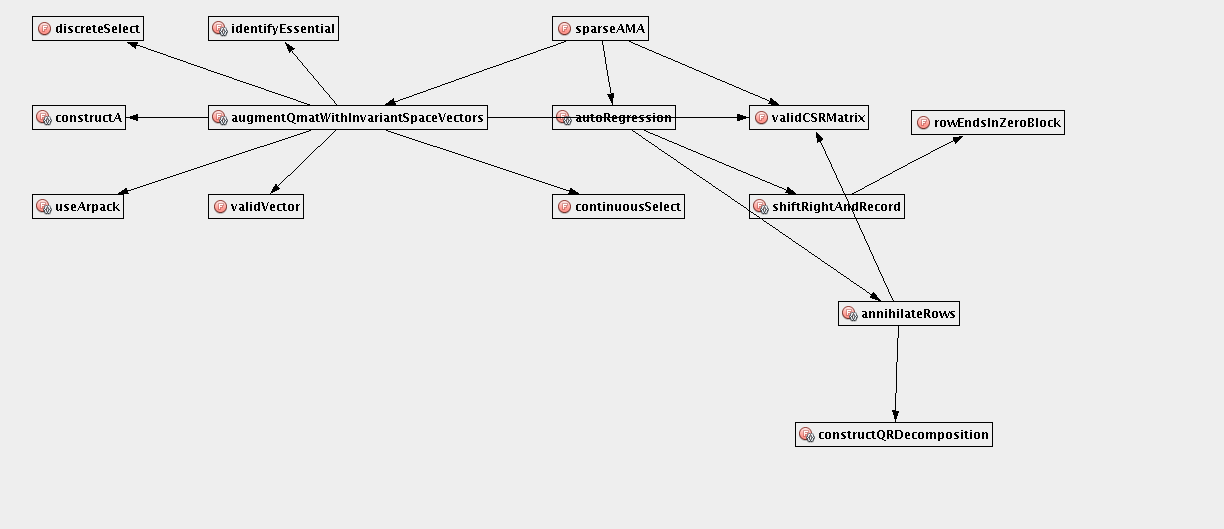
\includegraphics{sparseAMA.png}
\item problems with java versions mixing java 8 and java 7 in mvn call
\item had accidently made some directories in sparseAMA owned by root to build failed as non root
\item \href{https://www.codeproject.com/Articles/13853/Secure-Coding-Best-Practices-for-Memory-Allocation}{best practices for memory allocation and deallocation} Also some security implications
\item \href{http://stackoverflow.com/questions/5169692/assigning-negative-numbers-to-an-unsigned-int}{int to unsignedint}
\end{itemize}

\labday{Wednesday March 15, 2015}

\experiment{Parallel Programming}
\begin{itemize}
\item pose question to netbeans developers about transition to root ownership of target dir
  \begin{itemize}
  \item devise a simple example and run on mac and linux with java 7 and 8
  \end{itemize}
\item work on apple version rid of -Wall warnings and move to linux
\item get call graph for stackC and stochProto
\item fix useSparseAMA.h compileSparseAMA.h once and only once.
\item \href{http://www.network-theory.co.uk/docs/gccintro/gccintro_31.html}{more warnings possible}
\end{itemize}

\experiment{Administration}
\begin{itemize}
\item run netbeans with 8 or 7?
\item comcast
\end{itemize}

\labday{Thursday March 16, 2015}

\experiment{Parallel Programming}
\begin{itemize}
\item had maxNumberOfHelements instead of maxNumberOfHElements on argument list leading to segmentation violation.  Not sure why compiler -Wall did not catch this error. Worried that the text appears as a definition somewhere, but could not find it
\item want to get code in mathematica working to generate tests 
\item this would be best if it generates the admittedly more complicated code for
stackC and stochSims with the homotopy and other features
\end{itemize}
\subexperiment{get sparseAMA code in shape on laptop}
\begin{itemize}
\item runs the one test and simpleSparseAMAExample
\end{itemize}
\subexperiment{get sparseAMA code in shape on Linux}
\begin{itemize}
\item runs the one test and simpleSparseAMAExample
\end{itemize}

\begin{itemize}
\item choose java, 8 if possible  seems fine on laptop  Now using Java 8 laptop and linux
\item probably time to dump maven if it is not supported
\href{https://groups.google.com/forum/?fromgroups#!forum/maven-nar}{nar forum} seems it may be active  perhaps can develop in netbeans and archive and distribute in maven
\item \href{https://groups.google.com/d/msg/maven-nar/5feXpvN-Qh0/Sg3hAWgpwAcJ}{infor on netbeans directories and maven interaction}
\item make example to find out why netbeans has problems with gfortran on mac
\end{itemize}

\experiment{Administration}

\begin{itemize}
\item retirement details
\item calendar for events like retire/time to avoid reimburse for class
\item reviewintern applications
\item buy table after money arrives
\item give table away 
\item determine what to do with old table
\item balance accounts
\item FRB and other old data for balance accounts
\item need to update dependency checking in netbeans
\end{itemize}
\experiment{Machine Learning Application}

\begin{itemize}
\item develop seminar series economic applications
\item text categorization \href{https://www.federalreserve.gov/econresdata/notes/feds-notes/2015/semantic-analysis-of-the-FOMCs-postmeeting-statement-20150930.html}{Acosta and Meade}
\href{https://spweb.frb.gov/sites/ma/msu/FedCommunications/Wiki/Textual%20Analysis/Textual%20Analysis.aspx}{MSU}
\item \href{https://spweb.frb.gov/sites/ma/msu/FedCommunications/Wiki/Textual%20Analysis/Textual%20Analysis%20Data.aspx}{Textual Analysis Data Page}
  \item cleanNamedStatements.py contains code for preprocessing the docs including the ``stoplist'' of stop words  also removed numbers also n-grams to concatenate  (/msu/res1/www/Communications/Code\_Jupyter/data/)
This page is meant to be a place to store and share data used in textual analysis.  Much of the code from this website is available on the RSMA network at /msu/res1/www/Communications/Code\_Jupyter.  The data are available at /msu/res1/www/Communications/statements/Statement\_Alternatives and /msu/res1/www/Communications/statements/Statements\_Raw.
\item mathematica has a built-in wordstemmer using he porter clustering and \href{http://mathematica.stackexchange.com/questions/7441/k-means-clustering}{kmens}
\item should try stemming and using their stop words
\item \href{http://stackoverflow.com/questions/10554052/what-are-the-major-differences-and-benefits-of-porter-and-lancaster-stemming-alg}{porte vesus lancaster stemming}
\item stylistically FED employs synonyms instead of repeating
\item \href{https://spweb.frb.gov/sites/ma/msu/_layouts/15/xlviewer.aspx?id=/sites/ma/msu/MSU_Resources/list%20of%20words%20(increase%20and%20decrease).xlsx}{fed has list of synonyms}
 \item perhaps possible to use machine leaning to improve a formal grammar for the given domain
 \item\href{https://nlp.stanford.edu/software/lex-parser.shtml}{Stanford's statistical parser} \href{https://nlp.stanford.edu/software/lex-parser.shtml#Download}{parser download}
 \item \href{http://community.wolfram.com/groups/-/m/t/79795?p_p_auth=nEpA5pB6}{mma and word oriented tools}  Mentions nltk.or Language toolkit which appears to be what Ellen and Miguel used and something called WordData and ExampleData
 \item \href{http://community.wolfram.com/groups/-/m/t/227651?sortMsg=Flat}{synonym network in Mma}
 \item \href{https://www.wolfram.com/natural-language-understanding/}{Wolfram NL understanding system}
  \begin{itemize}
\item SOM visualization
  \end{itemize}

\end{itemize}

\experiment{Alena Collaboration}
  \begin{itemize}
  \item choose simplest cross validation and implement
  \end{itemize}
\experiment{AMA Series}
\begin{itemize}
\item univariate SVM function approx using libsvm
\end{itemize}



\labday{Friday March 17, 2015}
\experiment{Parallel Programming}
\begin{itemize}
\item want to get code in mathematica working to generate tests 
\item got sparseAMA and CStochSims code working switched to unsigned ints cstoch sims has seg fault
\item runing java 8 and netbeans 8.2 laptop and linux
\item using makefiles for now perhaps return to maven especially if firewall fix approved and I start using the stanford NLP see above for Nar fixes
\end{itemize}


\experiment{Administration}

\begin{itemize}
\item retirement details
\item calendar for events like retire/time to avoid reimburse for class
\item reviewintern applications
\item buy table after money arrives
\item giving table to courtney
\item balance accounts
\item FRB and other old data for balance accounts
\item need to update dependency checking in netbeans
\item use FRBFCU automate rent
\end{itemize}
\experiment{Machine Learning Application}
\begin{itemize}
\item develop seminar series economic applications
\item text categorization using Stanford NLP
\item SOM visualization
  \end{itemize}


\experiment{Alena Collaboration}
  \begin{itemize}
  \item choose simplest cross validation and implement
  \item sort out what intern will do
  \item example regression exercise to Alena
  \end{itemize}

\experiment{AMA Series}
\begin{itemize}
\item univariate SVM function approx using libsvm
\end{itemize}

\labday{Monday March 20, 2015}

\experiment{AMA Series}
\begin{itemize}
\item univariate SVM function approx using libsvm
\item CEF register TA
\end{itemize}

\experiment{Parallel Programming}
\begin{itemize}
\item mathematica code to generate tests
\item tests sparseAMA
\item sparseAMA cluster server solver tuned mpi
\item location of old sparseAim.w /msu/res2/m1gsa00/proj3/garyFiles/big/cFiles/nuwebTree/sparseAim.w
\item  found flow chart program flow and the inputs fpor AMA

/msu/res2/m1gsa00/aim/reliable/unconstrainedAR.flo
/msu/res2/m1gsa00/aim/reliable/test.flo
/msu/res2/m1gsa00/aim/reliable/convergenceConstraint.flo
/msu/res2/m1gsa00/aim/reliable/aimComponentsOverall.flo
/msu/res2/m1gsa00/aim/papers/description/unconstrainedAR.flo
/msu/res2/m1gsa00/aim/papers/description/test.flo
/msu/res2/m1gsa00/aim/papers/description/convergenceConstraint.flo
/msu/res2/m1gsa00/aim/papers/description/aimComponentsOverall.flo
/msu/res2/m1gsa00/algDesc/unconstrainedAR.flo
/msu/res2/m1gsa00/algDesc/test.flo
/msu/res2/m1gsa00/algDesc/convergenceConstraint.flo
/msu/res2/m1gsa00/algDesc/aimComponentsOverall.flo
\item compiled a ``safe'' version of flow using mkstemp instead of tmpnam
\item put notebook.sty in  git/paperProduction/texFiles
\end{itemize}

\experiment{Alena Collaboration}
\begin{itemize}
  \item choose simplest cross validation and implement
  \item sort out what intern will do
  \item example regression exercise to Alena
\item Summer Intern
\item clean up/simplify code for the intern to use
\end{itemize}

\experiment{Research Computing}

\begin{itemize}
\item plan seminar series
\end{itemize}


\experiment{Text Analysis}
\begin{itemize}
\item install Stanford Parser -done
\item example

export CLASSPATH=/msu/res5/software/stanford-parser-full-2016-10-31/stanford-parser.jar

java edu.stanford.nlp.process.PTBTokenizer /msu/res1/www/Communications/statements/Statements\_Raw/statement.fomc.20070321.txt

\item from README

/msu/res5/software/stanford-parser-full-2016-10-31/lexparser.sh /msu/res1/www/Communications/statements/Statements\_Raw/statement.fomc.20070321.txt
 runs out of memory on some o the parsers

\item  putting some statements in knowledgeXfer dir

cp /msu/res1/www/Communications/statements/Statements\_Raw/statement.fomc.20070321.txt  

/msu/res5/software/stanford-parser-full-2016-10-31/lexparser.sh statement.fomc.20070321.txt
\end{itemize}

\experiment{Administration}

\begin{itemize}
\item retirement options - emailed Flint meeting tomorrow
\item Avalon overpayment
\item booking room for NY SCE - done, but they will have to get back to me once they see the special rate  in their system
\item SCE plane tickets -- best wait till SED decision
\item robo form on iron key?  won't work due to firewall.  should recall scott fabri suggestion
\item progress on firewall mvn?
\end{itemize}

\labday{Tuesday March 21, 2017}
\experiment{stochastic simulations}

\begin{itemize}
\item tests tests tests
\item portable random numbers sprng U001 /msu/scratch2  dieharder pdh international?
\end{itemize}

\experiment{Administration}
\begin{itemize}
\item intern applications found one that looks good
\item roboform on iron key provides login help for board laptop and desktop without synch facility
\item investigate phased retirement
\end{itemize}

\labday{Wednesday, March 22, 2017}

\experiment{Stochastic Simulations}
\begin{itemize}
\item write tests  from sparseAMA through stochProto
\item dir to generate test example in symbolic math
/msu/home/m1gsa00/git/mathAMA/SymbolicAMA/SymbolicAMA/examples
\item cmath on cluster
\item taylor79  paper reference not very helpful in describing the model in taylor79.mth
\item best practice entail including unit tests with source
  \begin{itemize}
  \item can test private static methods
  \item can modify tests in same place/time  as code modified
  \end{itemize}

\end{itemize}

\experiment{Alena Collaboration}
\begin{itemize}
\item summer intern progress
\end{itemize}

\experiment{Administration}
\begin{itemize}
\item Alena laptop
\item power
\item sent plane info
\end{itemize}



\labday{Thursday, March 23, 2017}

\experiment{Stochastic Simulations}
\begin{itemize}
\item write tests  from sparseAMA through stochProto
\item using example dir to generate test example in symbolic math
/msu/home/m1gsa00/git/mathAMA/SymbolicAMA/SymbolicAMA/examples
\item cunit for sparseama tests in netbeans not done yet
\item use multiple suites one for each example model  -- two suites share variables need better exclusive names or maybe just make static
\item the file redo.sh runs on laptop and on linux
\end{itemize}

\experiment{Alena Collaboration}
\begin{itemize}
\item summer intern progress -- one contacted Bob lining up the other 4
\item use /msu/home/m1gsa00/git/svmrStuff/SVMRDesktop.nb 
\item hv-block cross validation
\end{itemize}

\experiment{AMA Series}
\begin{itemize}
\item do some work to refresh memory 
\item trying paperVerifyRBC.nb in git/AMASeriesRepresentation directories
\item no support for language English  needed to use babel to make fmtcount happy
\item found VerificationTest while looking for call graph for mathematica
\item linux notebook very very slow
\item try windows workbench  AMASeriesRep.nb in fixAMASeries workspace
\end{itemize}

\experiment{Research Computing Seminar Series}

\begin{itemize}
\item flesh out machine learning parallel programming talks
\item parallel computing on our cluster
  \begin{itemize}
  \item openmp and mpi
  \item overheads
  \item NUMA
  \item trends/future
  \end{itemize}
\end{itemize}

\experiment{Text Analysis}
\begin{itemize}
\item sort out training parser versus trained parser  what is output  what are features
\item SOM?
\item contact Ellen
\end{itemize}

\experiment{Administration}
\begin{itemize}
\item Alena laptop
\item power 
\item send last plane info
\item checking the recently installed swish-e on ubtest1   (ssh ubtest1)  
\end{itemize}

\labday{Friday, March 24, 2017}

\experiment{Stochastic Simulations}
\begin{itemize}
\item write tests  from sparseAMA through stochProto
\item cunit for sparseama tests in netbeans 
\item change names of test arrays
\item use multiple suites one for each example model  -- two suites share variables need better exclusive names or maybe just make static
\end{itemize}

\experiment{Alena Collaboration}
\begin{itemize}
\item summer intern progress -- one contacted Bob lining up the other 4
\item develop project outline for intern contribution
\item svmrCode.mth has  hv-cv {node001a,~/git/manchesterCS/61011/project,54}
\item my regression code is ~/git/svmrStuff/SVMR/SVMR.m
\end{itemize}

\experiment{AMA Series}
\begin{itemize}
\item construct call graph and tests 
\item trying paperVerifyRBC.nb in git/AMASeriesRepresentation directories

\item found VerificationTest while looking for call graph for mathematica
\item linux notebook very very slow
\item try windows workbench  AMASeriesRep.nb in fixAMASeries workspace
\item \href{https://reference.wolfram.com/language/ref/GraphPlot.html}{graphPlot} SpringEmbedding betterHighDimensionalEmbedding better RadialDrawing better than Circular or Random better than Linear
\item need t get rid of multiple arcs between same node
\end{itemize}

\experiment{Research Computing Seminar Series}

\begin{itemize}
\item flesh out machine learning parallel programming talks
\item parallel computing on our cluster
  \begin{itemize}
  \item openmp and mpi
  \item overheads
  \item NUMA
  \item trends/future
  \end{itemize}
\end{itemize}

\experiment{Text Analysis}
\begin{itemize}
\item sort out training parser versus trained parser  what is output  what are features
\item SOM?
\item contact Ellen
\end{itemize}

\experiment{Administration}
\begin{itemize}
\item Alena laptop
\item power 
\item checking the recently installed swish-e on ubtest1   (ssh ubtest1)  
\end{itemize}

\experiment{Retirement}
\begin{itemize}
\item Get numbers for 
  \begin{itemize}
  \item Bank Plan
  \item TIAA CREF
  \item Thrift Plan
  \end{itemize}
\item organize paperwork
\end{itemize}

\experiment{Quantum Computing}
\begin{itemize}
\item class
\item jobs
\item \href{https://www.reddit.com/r/askscience/comments/2egd6r/what_are_the_implications_for_quantum_computing/}{QC and linear algebra}
\item \href{https://www.dwavesys.com/careers/site-quantum-computing-expert}{QC Expert Dwave  DC}
\item \href{https://en.wikipedia.org/wiki/Quantum_finance}{Quantum finance}
\item \href{https://www.wired.com/2017/01/d-wave-turns-open-source-democratize-quantum-computing/}{dwave open sorce}
\item \href{http://community.wolfram.com/groups/-/m/t/897811}{wolfram language}
\item \href{http://homepage.cem.itesm.mx/jose.luis.gomez/quantum/}{Monterrey}
\item installed quantum package on  linux
\end{itemize}


\labday{Monday, March 27, 2017}

\experiment{Stochastic Simulations}
\begin{itemize}
\item cunit for sparseama tests in netbeans
  \begin{itemize}
  \item specifically connecting to c application not c++
  \item trying to set ldlibrarypath since netbeans complains not detected
  \end{itemize}

\item change names of test arrays
\item use multiple suites for each example model 
\item \href{http://stackoverflow.com/questions/19354321/integration-of-c-c-unit-test-with-maven}{maven and cunit}  no word from IT about maven since request of March 6
\item 
\end{itemize}

\experiment{Alena Collaboration}
\begin{itemize}
\item summer intern progress -- one contacted Bob lining up the other 4
\item develop project outline for intern contribution
\item svmrCode.mth has  hv-cv {node001a,~/git/manchesterCS/61011/project,54}
\item my regression code is ~/git/svmrStuff/SVMR/SVMR.m
\item at board use SVMRDesktop.nb in git/svmrStuff
\end{itemize}

\experiment{AMA Series}
\begin{itemize}
\item use  call start  tests 
\item trying paperVerifyRBC.nb in git/AMASeriesRepresentation directories
\item use VerificationTest 
\item linux notebook very very slow
\item get rid of multiple arcs between same node
\end{itemize}

\experiment{Research Computing Seminar Series}

\begin{itemize}
\item flesh out machine learning parallel programming talks
\item parallel computing on our cluster
  \begin{itemize}
  \item openmp and mpi
  \item overheads
  \item NUMA
  \item trends/future
  \end{itemize}
\end{itemize}

\experiment{Text Analysis}
\begin{itemize}
\item sort out training parser versus trained parser  what is output  what are features
\item SOM?
\item contact Ellen
\end{itemize}

\experiment{Administration}
\begin{itemize}
\item Alena laptop
\item downloaded symbolic C++
\item power 
\item checking the recently installed swish-e on ubtest1   (ssh ubtest1)  
\end{itemize}

\experiment{Retirement}
\begin{itemize}
\item Get numbers for 
  \begin{itemize}
  \item Bank Plan
  \item TIAA CREF
  \item Thrift Plan
  \end{itemize}
\item organize paperwork
\end{itemize}

\experiment{Quantum Computing}
\begin{itemize}
\item class
\item jobs
\end{itemize}


\labday{Tuesday, March 28, 2017}

\experiment{Stochastic Simulations}
\begin{itemize}
\item abandoning getting cunit to work pefectly in netbeans
  \item  set ldlibrarypath since netbeans complains cunit not detected. didn't help
\item changed names of test arrays
\item using multiple suites for each example model 
\end{itemize}

\experiment{Alena Collaboration}
\begin{itemize}
\item should sort out calling summer intern
Danno Thursday at 2
\item develop project outline for intern contribution
\item progress with hv validation  so far increasing h and v monotonically reduces the NMSE.  need to sort oout how to choose
\item my regression code is ~/git/svmrStuff/SVMR/SVMR.m
\item paper is ~/git/paperProduction/alenaCollab/docs/svmrRevisit
\item at board use SVMRDesktop.nb in git/svmrStuff
\item no definitive model selection/feature selection technique
\item hv Block no rigorous proof
\end{itemize}

\experiment{AMA Series}
\begin{itemize}
\item use  call graph start  tests 
\item trying paperVerifyRBC.nb in git/AMASeriesRepresentation directories  Couldn't get the suggestion to work for me 
\item fall back to use \href{http://reference.wolfram.com/language/guide/SystematicTestingAndVerification.html}{VerificationTest } in .w file
\item get rid of multiple arcs between same node
\end{itemize}

\experiment{Research Computing Seminar Series}

\begin{itemize}
\item flesh out machine learning parallel programming talks
\item parallel computing on our cluster
  \begin{itemize}
  \item openmp and mpi
  \item overheads
  \item NUMA
  \item trends/future
  \end{itemize}
\end{itemize}

\experiment{Text Analysis}
\begin{itemize}
\item sort out training parser versus trained parser  what is output  what are features
\item SOM?
\item contact Ellen
\end{itemize}

\experiment{Administration}
\begin{itemize}
\item Alena laptop
\item downloaded symbolic C++
\item power 
\item checking the recently installed swish-e on ubtest1   (ssh ubtest1)  
\end{itemize}

\experiment{Retirement}
\begin{itemize}
\item Get numbers for 
  \begin{itemize}
  \item Bank Plan
  \item TIAA CREF
  \item Thrift Plan
  \end{itemize}
\item organize paperwork
\end{itemize}

\experiment{Quantum Computing}
\begin{itemize}
\item class
\item jobs
\end{itemize}


\labday{Wednesday, March 29, 2017}

Too many projects on the agenda

\experiment{Stochastic Simulations}
\begin{itemize}
\item installed swish++ instead -- but did actually remove comments from code into verbatim and set up a couple of new tests for augmentq for one equation model
\end{itemize}

\experiment{Alena Collaboration}
\begin{itemize}
\item prepare summer intern talking points
\item develop project outline for intern contribution
\item how choose hv?
\end{itemize}

\experiment{AMA Series}
\begin{itemize}
\item use  call graph start  tests 
\item \item \href{http://mathematica.stackexchange.com/questions/54594/how-to-use-the-testing-notebook-to-test-a-package}{try test notebooks}
\item get rid of multiple arcs between same node
\end{itemize}

\experiment{Research Computing Seminar Series}

\begin{itemize}
\item flesh out machine learning parallel programming talks
\item parallel computing on our cluster
  \begin{itemize}
  \item openmp and mpi
  \item overheads
  \item NUMA
  \item trends/future
  \end{itemize}
\end{itemize}

\experiment{Text Analysis}
\begin{itemize}
\item sort out training parser versus trained parser  what is output  what are features
\item SOM?
\item contact Ellen
\end{itemize}

\experiment{Administration}
\begin{itemize}
\item try index   -v3 -i testIndexForDotM++ -c doDotM++  /msu/home/m1gsa00/git/paperProduction/SPSolveNot/ using /msu/res5/software/swish++-6.1.5/swish++.conf from installation as template 
\item apparently could have one index for all types of files
\item doing huge index started 12:13pm done by 1:30
index: done:
  70:07 (min:sec) elapsed time
  646633 files, 267372 indexed
  1852797849 words, 557879702 indexed, 5263645 unique

\item search   -i indexForDotM++ Package
\item need to figure out how to put in configuration file and specify multiple cirectors to make or huge search with complete coverage  (incremental index?)
\item Alena laptop
\end{itemize}

\experiment{Retirement}
\begin{itemize}
\item Looked at google england couple jobs look interesting
\item organize paperwork
\item apply job  -- contact  the name is Hal Varian not Villani
\end{itemize}

\experiment{Quantum Computing}
\begin{itemize}
\item class
\item jobs
\end{itemize}


\labday{Thursday, March 30, 2017}

Too many projects on the agenda

\experiment{Stochastic Simulations}
\begin{itemize}
\item do more sparseAMA tests using one equation
\item need to fix sparseAMAAssert linenumbers so lineNumberToString line 1221 reports correctly  )(it says line number but it appears to use error code which is accurate but not informative enough code does print file and line
\item do one equation where no shifts
\end{itemize}


\experiment{Alena Collaboration}
\begin{itemize}
\item prepare summer intern talking points
\item interview potential intern
\item develop project outline for intern contribution
\item how choose hv?  write up
\end{itemize}

\experiment{AMA Series}
\begin{itemize}
\item continue adding tests
\item get rid of multiple arcs between same node
\item get started on multivariate svmr
\end{itemize}

\experiment{Research Computing Seminar Series}

\begin{itemize}
\item flesh out machine learning parallel programming talks
\item parallel computing on our cluster
  \begin{itemize}
  \item openmp and mpi
  \item overheads
  \item NUMA
  \item trends/future
  \end{itemize}
\item organize as mathematica notebooks?
\item use the papers Alena, AMASeries and Text Analysis to generate applications
\end{itemize}

\experiment{Text Analysis}
\begin{itemize}
\item sort out training parser versus trained parser  what is output  what are features
\item SOM?
\item contact Ellen
\end{itemize}

\experiment{Administration}
\begin{itemize}
\item need to figure out how to put in configuration file and specify multiple cirectors to make or huge search with complete coverage  (incremental index?)
\item Alena laptop
\end{itemize}

\experiment{Retirement}
\begin{itemize}
\item Looked at google england couple jobs look interesting
\item organize paperwork
\item apply job  -- 
\item emailed and linked in  Hal Varian 
\end{itemize}

\experiment{Quantum Computing}
\begin{itemize}
\item class
\item jobs
\end{itemize}

\experiment{Referee}
\begin{itemize}
\item paper "Can we Identify the Fed's Preferences?," by Jean-Bernard Chatelain and Kirsten Ralf, which I am handling as an Associate Editor for Macroeconomic Dynamics 
\end{itemize}

\labday{Friday, March 31, 2017}

Too many projects on the agenda

\experiment{Stochastic Simulations}
\begin{itemize}
\item do more sparseAMA tests using one equation
\item generate test matrice as .mat files from steps in spsolve
\item read .mat into c \href{http://www.mathworks.com/help/matlab/matlab_external/_f30937.html}{.mat}
\item need to fix sparseAMAAssert linenumbers so lineNumberToString line 1221 reports correctly  )(it says line number but it appears to use error code which is accurate but not informative enough code does print file and line
\item do one equation where no shifts
\item interactive version of SPAMA operation  (jupyter)
\end{itemize}


\experiment{Alena Collaboration}
\begin{itemize}
\item prepare summer intern talking points
\item interview potential interns  Danno Lemu and Neal Dora
\item develop project outline for intern contribution
\item how choose hv?  write up
\end{itemize}

\experiment{AMA Series}
\begin{itemize}
\item continue adding tests
\item get rid of multiple arcs between same node
\item get started on multivariate svmr
\end{itemize}

\experiment{Research Computing Seminar Series}

\begin{itemize}
\item flesh out machine learning parallel programming talks
\item parallel computing on our cluster
  \begin{itemize}
  \item openmp and mpi
  \item overheads
  \item NUMA
  \item trends/future
  \end{itemize}
\item organize as mathematica notebooks?
\item use the papers Alena, AMASeries and Text Analysis to generate applications
\end{itemize}

\experiment{Text Analysis}
\begin{itemize}
\item sort out training parser versus trained parser  what is output  what are features
\item SOM?  probably best to use matlab som from manchester
\item contact Ellen
\end{itemize}

\experiment{Administration}
\begin{itemize}
\item figured out how to put in configuration file and specify multiple cirectors  look at search nuiance
\item Alena laptop
\item investigate vivify scrum \href{https://www.vivifyscrum.com/feature/how-it-works}{using basic but will probably upgrade find out owned versus access}
\end{itemize}

\experiment{Retirement}
\begin{itemize}
\item Looked at google england couple jobs look interesting
\item organize paperwork
\item apply job  -- 
\end{itemize}

\experiment{Quantum Computing}
\begin{itemize}
\item class
\item jobs vita  cover
\item visa
\item dwave uses linear algebra?  ``adibatic?''
\end{itemize}

\experiment{Referee}
\begin{itemize}
\item decide paper "Can we Identify the Fed's Preferences?," by Jean-Bernard Chatelain and Kirsten Ralf, which I am handling as an Associate Editor for Macroeconomic Dynamics 
\end{itemize}


\labday{Saturday, April 1, 2017}

Too many projects on the agenda. Start using vivifyscrum KanBan style

\experiment{Stochastic Simulations}
\begin{itemize}
\item do more sparseAMA tests using one equation
\item generate test matrice as .mat files from steps in spsolve
\item read .mat into c \href{http://www.mathworks.com/help/matlab/matlab_external/_f30937.html}{.mat}
\item need to fix sparseAMAAssert linenumbers so lineNumberToString line 1221 reports correctly  )(it says line number but it appears to use error code which is accurate but not informative enough code does print file and line
\item do one equation where no shifts
\item interactive version of SPAMA operation  (jupyter)
\item use matio already installed on /msu/res1/  example use ~/git/sparseAMADesktop/
\item newer version of matio 1.5.10 can handle newer .mat files but requires getting other downloads
\item install matio on mac
\end{itemize}


\experiment{Alena Collaboration}
\begin{itemize}
\item prepare summer intern talking points
\item interview potential interns  Danno Lemu and Neal Dora
\item develop project outline for intern contribution
\item how choose hv?  write up
\end{itemize}

\experiment{AMA Series}
\begin{itemize}
\item continue adding tests
\item get rid of multiple arcs between same node
\item get started on multivariate svmr
\end{itemize}

\experiment{Research Computing Seminar Series}

\begin{itemize}
\item flesh out machine learning parallel programming talks
\item parallel computing on our cluster
  \begin{itemize}
  \item openmp and mpi
  \item overheads
  \item NUMA
  \item trends/future
  \end{itemize}
\item organize as mathematica notebooks?
\item use the papers Alena, AMASeries and Text Analysis to generate applications
\end{itemize}

\experiment{Text Analysis}
\begin{itemize}
\item sort out training parser versus trained parser  what is output  what are features
\item SOM?  probably best to use matlab som from manchester
\item contact Ellen
\end{itemize}

\experiment{Administration}
\begin{itemize}
\item figured out how to put in configuration file and specify multiple cirectors  look at search nuiance
\item Alena laptop
\item investigate vivify scrum \href{https://www.vivifyscrum.com/feature/how-it-works}{using basic but will probably upgrade find out owned versus access}
\end{itemize}

\experiment{Retirement}
\begin{itemize}
\item Looked at google england couple jobs look interesting
\item organize paperwork
\item apply job  -- 
\end{itemize}

\experiment{Quantum Computing}
\begin{itemize}
\item class
\item jobs vita  cover
\item visa
\item dwave uses linear algebra?  ``adibatic?''
\item \href{https://www.dwavesys.com/sites/default/files/Map%20Coloring%20WP2.pdf}{dwave map coloring}
\end{itemize}

\experiment{Referee}
\begin{itemize}
\item decide paper "Can we Identify the Fed's Preferences?," by Jean-Bernard Chatelain and Kirsten Ralf, which I am handling as an Associate Editor for Macroeconomic Dynamics 
\end{itemize}

\labday{Sunday, April 2, 2017}

Too many projects on the agenda. Start using vivifyscrum KanBan style

\experiment{Stochastic Simulations}
\begin{itemize}
\item do more sparseAMA tests using one equation
\item need to fix sparseAMAAssert linenumbers so lineNumberToString line 1221 reports correctly  )(it says line number but it appears to use error code which is accurate but not informative enough code does print file and line
\item interactive version of SPAMA operation  (jupyter)
\item newer version of matio 1.5.10 can handle newer .mat files but requires getting other downloads
\end{itemize}


\experiment{Alena Collaboration}
\begin{itemize}
\item develop project outline for intern contribution
\item how choose hv?  write up
\end{itemize}

\experiment{AMA Series}
\begin{itemize}
\item continue adding tests
\item get rid of multiple arcs between same node
\item get started on multivariate svmr
\end{itemize}

\experiment{Research Computing Seminar Series}

\begin{itemize}
\item flesh out machine learning parallel programming talks
\item parallel computing on our cluster
  \begin{itemize}
  \item openmp and mpi
  \item overheads
  \item NUMA
  \item trends/future
  \end{itemize}
\item organize as mathematica notebooks?
\item use the papers Alena, AMASeries and Text Analysis to generate applications
\end{itemize}

\experiment{Text Analysis}
\begin{itemize}
\item sort out training parser versus trained parser  what is output  what are features
\item learn matlab SOM
  \begin{itemize}
  \item demos in  ~/git/manchesterCS/61021/week9/lab2\_Part2
  \item alenas data in ~/git/manchesterCS/61011/alenaMatlabCode,
  \end{itemize}

\item contact Ellen
\end{itemize}

\experiment{Administration}
\begin{itemize}
\item learn new swish search
\item Alena laptop
\end{itemize}

\experiment{Retirement}
\begin{itemize}
\item Looked at google england couple jobs look interesting
\item organize paperwork
\item apply job  -- 
\end{itemize}

\experiment{Quantum Computing}
\begin{itemize}
\item class
\item jobs vita  cover  in planning
\item visa
\item dwave uses linear algebra?  ``adibatic?''
\item \href{https://www.dwavesys.com/sites/default/files/Map%20Coloring%20WP2.pdf}{dwave map coloring}
\end{itemize}

\labday{Monday, April 3, 2017}

\experiment{Stochastic Simulations}
\begin{itemize}
\item stack.m work
\end{itemize}


\experiment{Alena Collaboration}
\begin{itemize}
\item develop project outline for intern contribution
\item how choose hv?  write up
\end{itemize}

\experiment{AMA Series}
\begin{itemize}
\item continue adding tests
\item get rid of multiple arcs between same node
\item get started on multivariate svmr
\end{itemize}

\experiment{Research Computing Seminar Series}

\begin{itemize}
\item flesh out machine learning parallel programming talks
\item parallel computing on our cluster
  \begin{itemize}
  \item openmp and mpi
  \item overheads
  \item NUMA
  \item trends/future
  \end{itemize}
\item organize as mathematica notebooks?
\item use the papers Alena, AMASeries and Text Analysis to generate applications
\end{itemize}

\experiment{Text Analysis}
\begin{itemize}
\item sort out training parser versus trained parser  what is output  what are features
\item learn matlab SOM
  \begin{itemize}
  \item demos in  ~/git/manchesterCS/61021/week9/lab2\_Part2
  \item alenas data in ~/git/manchesterCS/61011/alenaMatlabCode,
  \end{itemize}

\item contact Ellen
\end{itemize}

\experiment{Administration}
\begin{itemize}
\item learn new swish search
\item Alena laptop
\end{itemize}

\experiment{Retirement}
\begin{itemize}
\item Looked at google england couple jobs look interesting
\item organize paperwork
\item apply job  -- 
\end{itemize}

\experiment{Quantum Computing}
\begin{itemize}
\item class
\item jobs vita  cover  in planning
\item visa
\item dwave uses linear algebra?  ``adibatic?''
\item \href{https://www.dwavesys.com/sites/default/files/Map%20Coloring%20WP2.pdf}{dwave map coloring}
\end{itemize}

\labday{Monday, April 3, 2017}

Start including only new info and accomplishments.


\experiment{Stochastic Simulations}
\begin{itemize}
\item to implement stack need submatrix zeromatrix  blockmatrix asymptoticlinearization
\item mathAMA/SymbolicAMA/SymbolicAMA/SymbolicAMA.m has submatrix zeromatrix  blockmatrix 
\item amsMatrices used by stochProtoTest.m  ./experFRBUSMPS/amsMatrices.m
./stackStochSimsNot/amsMatrices.m
\item /msu/res2/m1gsa00/dirDevConvergence/convergence/src/mathematica/asymptotic/asymptoticLinearization.w 
\item put AsymptoticLinearization in ~/git/CStochSims/reMakeStackMma/
\item much of stack.w works -- see testStack.m (i think the errors are from my executing commands in random order and mixing models
\item can even generate spliced c file
\item homotopy in /msu/res2/m1gsa00/proj3/garyFiles/big/cFiles/nuwebTree/compXEtm1.c

\end{itemize}


\experiment{Alena Collaboration}
\begin{itemize}
\item 
\end{itemize}

\experiment{AMA Series}
\begin{itemize}
\item 
\end{itemize}

\experiment{Research Computing Seminar Series}

\begin{itemize}
\item 
\end{itemize}

\experiment{Text Analysis}
\begin{itemize}
\item
\end{itemize}

\experiment{Administration}
\begin{itemize}
\item 
\end{itemize}

\experiment{Retirement}
\begin{itemize}
\item \href{http://rpi.edu/dept/arc/training/latex/resumes/}{resume and letter templates}
\item europass looks nice and sanctioned by the EU
\end{itemize}

\experiment{Quantum Computing}
\begin{itemize}
\item 
\end{itemize}



\labday{Wednesday, April 5, 2017}

Start including only new info and accomplishments.


\experiment{Stochastic Simulations}
\begin{itemize}
\item to generate code work with toggle.mth in git/doToggle directory
\item toggle.mth calls for Stoch` and Stack` present in /msu/home/m1gsa00/git/stackStochSimsNot/
\item doToggle geneates rbc.mod .xml and .mth
\item doToggle seems to work with Stack and Stoch from /msu/home/m1gsa00/git/stackStochSimsNot/
\item even stochSim[2, 2, 9, rbcTestModel, 1, t] // Chop // TableForm seems to work
\item then run rbcGenCc.mth but fails with problems from dense to sparse mat
\item doSplice not defined perhaps not needed
\item generateCCode has problems with dens conversion in
/msu/home/m1gsa00/git/stackStochSimsNot/MmaModelToC.m
\item SymbolicAMA has denseToSparseMat as well as Stack
even though it needs symbolicAMA  mmamodeltoc didn't have need symbolicAMA
\item following seems to work on cluster

  \begin{enumerate}
  \item cd /msu/home/m1gsa00/git/doToggle
  \item cmath
  \item Get["toggle.mth"] 
  \item Get["rbcGenC.mth"]
  \end{enumerate}
\item had to comment out defs in Stack and add SymbolicAMA to needs of MmaModelToC
\item move all code to CStochSims and simplify use Stack and Stoch
\item GenStochSimsExample.m   starts with rbcChk.in.xml(mq style model file)  generates c for stoch sims  Get["useGenStochSimsExample.mth"]
\item model to c now generates code for the homotopy version

\end{itemize}


% \experiment{Alena Collaboration}
% \begin{itemize}
% \item 
% \end{itemize}

% \experiment{AMA Series}
% \begin{itemize}
% \item 
% \end{itemize}

% \experiment{Research Computing Seminar Series}

% \begin{itemize}
% \item 
% \end{itemize}

% \experiment{Text Analysis}
% \begin{itemize}
% \item
% \end{itemize}

% \experiment{Administration}
% \begin{itemize}
% \item 
% \end{itemize}

% \experiment{Retirement}
% \begin{itemize}
% \item 
% \end{itemize}

% \experiment{Quantum Computing}
% \begin{itemize}
% \item 

% \end{itemize}


\labday{Thursday, April 6, 2017}




\experiment{Stochastic Simulations}
\begin{itemize}


\item compile warnings for generated c files. Placed originals in originalGenC 
so can update to get rid of warnings and retrieve differences without putting i repository in file warnings.tex. 
\item added to git anyway so can send to mac
  % \listinginput{1}{warnings.tex}  cause latex error if included

\item lots of diffs so will try call graph in netbeans to see chain from main down to model evaluation
%
%\item \includegraphics[width=6in]{/msu/home/m1gsa00/git/CStochSims/fpnewt.png}
%\item \includegraphics[width=6in]{/msu/home/m1gsa00/git/CStochSims/stochsim.png}
\item to see call graph click on function name in a .c file not a .w file
\item allocFPNewt not used?  probably should be
\item had implemented a method for exogenizing rows and columns
  \begin{itemize}
  \item look in  directory /msu/res2/m1gsa00/proj3/garyFiles/big/cFiles/nuwebTree/toRay041702/aimver/
  \item I think exogenizing zeroes out impact of equations and lets just the shocks show through
  \end{itemize}
\end{itemize}


% \experiment{Alena Collaboration}
% \begin{itemize}
% \item 
% \end{itemize}

% \experiment{AMA Series}
% \begin{itemize}
% \item 
% \end{itemize}

% \experiment{Research Computing Seminar Series}

% \begin{itemize}
% \item 
% \end{itemize}

% \experiment{Text Analysis}
% \begin{itemize}
% \item
% \end{itemize}

% \experiment{Administration}
% \begin{itemize}
% \item 
% \end{itemize}

% \experiment{Retirement}
% \begin{itemize}
% \item 
% \end{itemize}

% \experiment{Quantum Computing}
% \begin{itemize}
% \item 
% \end{itemize}



\labday{Friday, April 7, 2017}




\experiment{Stochastic Simulations}
\begin{itemize}
\item some ideas from dinner
\item Could communicate seed and step instead is sending shocks
\item Granularity of task for work stealing.  1 step or multi step
\item Also Think about appropriate draws from history.  Look at parallel bootstrap applications
\item  Cilk gpu?
\item \href{http://paralleltasks.codeplex.com/}{work steal scheduling}
\end{itemize}


% \experiment{Alena Collaboration}
% \begin{itemize}
% \item 
% \end{itemize}

% \experiment{AMA Series}
% \begin{itemize}
% \item 
% \end{itemize}

% \experiment{Research Computing Seminar Series}

 \begin{itemize}
 \item compile info about cluster ~/git/manchesterCS/knowledgeXfer/clusterParallel.tex
 \item node001d snapshot into practicalSteps paper
 \end{itemize}

 \experiment{Text Analysis}
 \begin{itemize}
 \item ~/git/manchesterCS/knowledgeXfer/textAnalysis
 \end{itemize}

 \experiment{Administration}
 \begin{itemize}
 \item swish file became zero length some how. must have accidentally started reindex and aborted
 \item getting bus error when I reindex
 \end{itemize}

% \experiment{Retirement}
% \begin{itemize}
% \item 
% \end{itemize}

% \experiment{Quantum Computing}
% \begin{itemize}
% \item 
% \end{itemize}






\labday{Saturday, April 8, 2017}




\experiment{Stochastic Simulations}
\begin{itemize}
\item incorporate exogenizeQ at some point soon from /msu/res2/m1gsa00/proj3/garyFiles/big/cFiles/nuwebTree/stackC.w
\item should find memory leaks
\item pick optimization level
\item xml file all the info for selecting equations?
\end{itemize}


% \experiment{Alena Collaboration}
% \begin{itemize}
% \item 
% \end{itemize}

% \experiment{AMA Series}
% \begin{itemize}
% \item 
% \end{itemize}

% \experiment{Research Computing Seminar Series}

 \begin{itemize}
 \item compile info about cluster ~/git/manchesterCS/knowledgeXfer/clusterParallel.tex
 \item node001d snapshot into practicalSteps paper
 \end{itemize}

 \experiment{Text Analysis}
 \begin{itemize}
 \item ~/git/manchesterCS/knowledgeXfer/textAnalysis
 \end{itemize}

 \experiment{Administration}
 \begin{itemize}
 \item swish file became zero length some how. must have accidentally started reindex and aborted
 \item getting bus error when I reindex
 \end{itemize}

% \experiment{Retirement}
% \begin{itemize}
% \item 
% \end{itemize}

% \experiment{Quantum Computing}
% \begin{itemize}
% \item 
% \end{itemize}



\labday{Saturday, April 8, 2017}




\experiment{Stochastic Simulations}
\begin{itemize}
\item worked on incorporating full functionality on a git flow branch
\item feels like I am piece by piece incorporating all of the nuweb code
\item generated csr format with j and i interchanged 
\end{itemize}


 \experiment{Alena Collaboration}
 \begin{itemize}
 \item paper here ~/git/paperProduction/alenaCollab/docs/svmrRevisit.tex
 \end{itemize}

% \experiment{AMA Series}
% \begin{itemize}
% \item 
% \end{itemize}

 \experiment{Research Computing Seminar Series}

 \begin{itemize}
 \item \href{http://www.mellanox.com/pdf/whitepapers/Intro_to_IB_for_End_Users.pdf}{infiniband white paper}
 \end{itemize}

 \experiment{Text Analysis}
 \begin{itemize}
 \item 
 \end{itemize}

 \experiment{Administration}
 \begin{itemize}
 \item read cvs for summer interns  ~/planning/summerIntern2017/readCVs.tex
 \end{itemize}

% \experiment{Retirement}
% \begin{itemize}
% \item 
% \end{itemize}

% \experiment{Quantum Computing}
% \begin{itemize}
% \item 
% \end{itemize}





\labday{Monday, April 10, 2017}




\experiment{Stochastic Simulations}
\begin{itemize}
\item seems like a stupid error in stackC.w where I initialize a negative I matrix and then pass the wrong pointer to matrix to nxtcdmats.  hard to see how it might ever have worked with this error
\item useGenStochSimsExample.mth seems to work, but overwrites updated .c files
\item probably need to update the code generators so that these cooperate
\end{itemize}


 \experiment{Alena Collaboration}
 % \begin{itemize}
 % \item 
 % \end{itemize}

% \experiment{AMA Series}
% \begin{itemize}
% \item 
% \end{itemize}

 \experiment{Research Computing Seminar Series}

 % \begin{itemize}
 % \item 
 % \end{itemize}



 \experiment{Text Analysis}
 % \begin{itemize}
 % \item 
 % \end{itemize}

 \experiment{Administration}
 % \begin{itemize}
 % \item 
 % \end{itemize}

% \experiment{Retirement}
% \begin{itemize}
% \item 
% \end{itemize}

% \experiment{Quantum Computing}
% \begin{itemize}
% \item 
% \end{itemize}






\labday{Tuesday, April 11, 2017}




\experiment{Stochastic Simulations}
\begin{itemize}
\item valgrind --tool=memcheck --leak-check=yes --show-reachable=yes --num-callers=20 --track-fds=yes ./runrbcTryC works on linux
\item Get["useStack.mth"] loadss Stack` and Stoch` 
Out[3]= {Stoch`, AMAModelDefinition`, Stack`, SymbolicAMA`, 
>    AsymptoticLinearization`, ProtectedSymbols`, 
>    SymbolicMachineLearningLoader`, StreamingLoader`, NeuralNetworks`,  
>    IconizeLoader`, HTTPHandlingLoader`, CloudObjectLoader`, PacletManager`, 
 >    System`, Global`}
\item stochProtoTest appears to work to do stoch sims

\end{itemize}


 \experiment{Alena Collaboration}
 % \begin{itemize}
 % \item 
 % \end{itemize}

% \experiment{AMA Series}
% \begin{itemize}
% \item 
% \end{itemize}

 \experiment{Research Computing Seminar Series}

 % \begin{itemize}
 % \item 
 % \end{itemize}



 \experiment{Text Analysis}
  \begin{itemize}
  \item Sharpe Seminar used tf-idf weight tonality measure from word count
  \end{itemize}

 \experiment{Administration}
  \begin{itemize}
  \item Sent Bob Burian my top 5 list.  Had Jason Osajima first who I already  have interviewed  but no way to leave 1st position blank on the  \href{https://fweb.rsma.frb.gov/add/intern_recruiting_2017/cgi-bin/recruiter_view.pl}{recruiter web page }
  \end{itemize}

 \experiment{Retirement}
 \begin{itemize}
 \item \href{https://careers.google.com/jobs#!t=jo&jid=/google/quantitative-analyst-1-13-st-giles-high-st-london-uk-2518841243&}{london}
 \end{itemize}

 \experiment{Quantum Computing}
% \begin{itemize}
% \item 
% \end{itemize}






\labday{Thursday, April 13, 2017}




\experiment{Stochastic Simulations}
\begin{itemize}
\item Get["MmaModelToC`"];Get["useGenStochSimsExample.mth"] reloads model c code generator and generates new rbcTryC
\item adapting stochProtoTest to  to do stoch sims for rbc in rbcStochSims.mth
\item useGen...  sets up rbc model equation
\item stochSim[2, 2, 1, rbcTestModel, 1, t] works already
\item Stack`Private`nxtFpGuess[Private`nlag, Private`theFunc, Private`theDrvFunc, guess]
\end{itemize}


 \experiment{Alena Collaboration}
 % \begin{itemize}
 % \item 
 % \end{itemize}

% \experiment{AMA Series}
% \begin{itemize}
% \item 
% \end{itemize}

 \experiment{Research Computing Seminar Series}

 % \begin{itemize}
 % \item 
 % \end{itemize}



 \experiment{Text Analysis}
  \begin{itemize}
  \item Sharpe Seminar used tf-idf weight tonality measure from word count
  \end{itemize}

 \experiment{Administration}
  \begin{itemize}
  \item Sent Bob Burian my top 5 list.  Had Jason Osajima first who I already  have interviewed  but no way to leave 1st position blank on the  \href{https://fweb.rsma.frb.gov/add/intern_recruiting_2017/cgi-bin/recruiter_view.pl}{recruiter web page }
  \end{itemize}

 \experiment{Retirement}
 \begin{itemize}
 \item \href{https://careers.google.com/jobs#!t=jo&jid=/google/quantitative-analyst-1-13-st-giles-high-st-london-uk-2518841243&}{london}
 \end{itemize}

 \experiment{Quantum Computing}
% \begin{itemize}
% \item 
% \end{itemize}








\labday{Friday, April 14, 2017}




\experiment{Stochastic Simulations}
\begin{itemize}
\item need to change the makefile since new stochProto doesn't make a stpochProto.c but instead 

-rw-r--r-- 1 m1gsa00 msu  9967 Apr 14 16:52 stochRun.c
-rw-r--r-- 1 m1gsa00 msu   916 Apr 14 16:54 compXEtm1.c
-rw-r--r-- 1 m1gsa00 msu  1172 Apr 14 16:54 generateNextXTMinusOne.c
-rw-r--r-- 1 m1gsa00 msu   545 Apr 14 16:54 generateDraws.c
-rw-r--r-- 1 m1gsa00 msu   792 Apr 14 16:54 generatePathX.c
-rw-r--r-- 1 m1gsa00 msu  1507 Apr 14 16:54 stochSims.c
-rw-r--r-- 1 m1gsa00 msu   570 Apr 14 16:55 stochSims.h
-rw-r--r-- 1 m1gsa00 msu 51300 Apr 14 17:58 myNewt.c
-rw-r--r-- 1 m1gsa00 msu  3081 Apr 14 17:58 stackC.h
-rw-r--r-- 1 m1gsa00 msu 51179 Apr 14 17:58 stackC.c
\begin{verbatim}

{msulx1,~/git/CStochSims,62}$grep ims.h *.c




compXEtm1.c:#include "stochSims.h"  from stochProto.w
generateDraws.c:#include "stochSims.h"from stochProto.w
generateNextXTMinusOne.c:#include "stochSims.h" from stochProto.w
generatePathX.c:#include "stochSims.h"from stochProto.w
myNewt.c:#include "stochSims.h"from stackC.w
runmpirbcTryC.c:#include "distStochSims.h"
stackC.c:#include "stochSims.h"from stackC.w
stackC.c:#include "stochSims.h"from stackC.w
stochSims.c:#include "stochSims.h"from stochProto.w
{msulx1,~/git/CStochSims,63}$

\end{verbatim}


\item for some reason have to quit mma and run Get["use..."] in order to get all the c files.

\item need to get nuweb dependencies righ
\item eliminate stochProto.w  just need stackC.w stochSims.w to make the libstochsims.a in makefile
\item nuweb stackC;nuweb stochSims;make clean; make libstochSims.a   
\end{itemize}



 \experiment{Alena Collaboration}
 % \begin{itemize}
 % \item 
 % \end{itemize}

% \experiment{AMA Series}
% \begin{itemize}
% \item 
% \end{itemize}

 \experiment{Research Computing Seminar Series}

 % \begin{itemize}
 % \item 
 % \end{itemize}



 \experiment{Text Analysis}
  \begin{itemize}
  \item 
  \end{itemize}

 \experiment{Administration}
  \begin{itemize}
  \item 
  \end{itemize}

 \experiment{Retirement}
 \begin{itemize}
 \item 
 \end{itemize}

 \experiment{Quantum Computing}
% \begin{itemize}
% \item 
% \end{itemize}



\labday{Friday, April 14, 2017}




 \experiment{Stochastic Simulations}
 \begin{itemize}
 \item re-running  
   does not produce c code

 \item    below no computing stedy state subs and loading all  but okay since if statement checks to see if exists already

 \item    probably Needs["GenStochSimsExample`"] is the issue
   
 \item adding Get["GenStochSimsExample`"] apparently does nothing
 \item need to close the OutputStreams associated with the target .[ch] files
 \item closing works for most but several have error on not open
   
General::openx: rbcTryCDrv.c is not open.

General::openx: rbcTryCMakefile is not open.

General::openx: rbcTryCDataForInclude.h is not open.

\begin{verbatim}
bash-3.2$ math
Mathematica 11.1.0 Kernel for Mac OS X x86 (64-bit)
Copyright 1988-2017 Wolfram Research, Inc.
reading from ~/Library/Mathematica/Kernel/init.m
fix for emacs
setting c compiler info

In[1]:= Get["useGenStochSimsExample.mth"]
done reading SymbolicAMA
done reading NumericAMA
done reading AMAModel
done reading AccelerateAMA
done reading AsymptoticLinearization
preprivate
before reading Format and Optimize
done reading Format and Optimize
doing assigns in mmaToC.m
{in private:, Private`, private}
sparseFunctionAssignments
done reading MmaModelToC.m
executing code for rbcChk.in.xml example
take care with names since
 cnstrctDModel appends to xxx.mod and
 parsemod overwrites xxx.xml
Current dir after this:/Users/garyanderson
Current dir using System  after this:/Users/garyanderson
computing steady state subs
done computing steady state subs
got hmatRBC
avoidSeries:about to compute product
csrToSpmat:starting
csrToSpmat:starting

In[2]:= Get["useGenStochSimsExample.mth"]
executing code for rbcChk.in.xml example
take care with names since
 cnstrctDModel appends to xxx.mod and
 parsemod overwrites xxx.xml
Current dir after this:/Users/garyanderson
Current dir using System  after this:/Users/garyanderson
got hmatRBC
avoidSeries:about to compute product
csrToSpmat:starting
csrToSpmat:starting

In[3]:= 
\end{verbatim}
 \end{itemize}



 \experiment{Alena Collaboration}
 % \begin{itemize}
 % \item 
 % \end{itemize}

 \experiment{AMA Series}
% \begin{itemize}
% \item 
% \end{itemize}

 \experiment{Research Computing Seminar Series}

 % \begin{itemize}
 % \item 
 % \end{itemize}



 \experiment{Text Analysis}
  % \begin{itemize}
  % \item 
  % \end{itemize}

 \experiment{Administration}
  % \begin{itemize}
  % \item 
  % \end{itemize}

 \experiment{Retirement}
 % \begin{itemize}
 % \item 
 % \end{itemize}

 \experiment{Quantum Computing}
% \begin{itemize}
% \item 
% \end{itemize}



\labday{Friday, April 28, 2017}

\begin{itemize}
\item  --ansi --strict 
\end{itemize}

\labday{Saturday, April 29, 2017}
\begin{itemize}
\item should include .w dependencies in makefile for runrbcTryC
\item \href{http://www.learncpp.com}{learn C++}
\end{itemize}

\labday{Monday, May 1, 2017}

  \begin{itemize}
  \item \href{http://www.cplusplus.com/reference/random/uniform_int_distribution/}{c++ uniform distribution}
  \item if no parameters will need to tell compiler unused variables parameters to avoid warning
  \end{itemize}
\labday{Tuesday, May 2, 2017}

\experiment{stochastic sims}
  \begin{itemize}
  \item eliminated warnings except for fortran 
  \item should eliminate ranlib.f reference
  \end{itemize}
\experiment{Alena collaboration}
\begin{itemize}
\item MATLink for linux  no anomalies for MEX 5  13 results except for coefficients which produce 12 since random walk has no coefficients
\item in emacs .m file get edited in matlab mode.  need a way to turn off for mathematica files
\end{itemize}


\experiment{Summer Intern}
\href{http://karpathy.github.io/2015/05/21/rnn-effectiveness/}{The Unreasonable Effectiveness of Recurrent Neural Networks}  also look at the Long Short-Term Memory network variant
\begin{itemize}
\item \href{http://torch.ch/}{torch}
\item \href{http://fastml.com/torch-vs-theano/}{Theano vs Torch}
\item \href{https://chunml.github.io/ChunML.github.io/project/Creating-Text-Generator-Using-Recurrent-Neural-Network/}{text generation RNN and ltsm}
\item \href{http://machinelearningmastery.com/text-generation-lstm-recurrent-neural-networks-python-keras/}{python LTSM}
\item \href{https://medium.com/@TalPerry/deep-learning-the-stock-market-df853d139e02}{,pre LSTM}
\item \href{https://ehudreiter.com/2016/12/12/nlg-and-ml/}{long time practitioner blog}
\end{itemize}

\labday{Friday, May 5, 2017}

\experiment{stochastic Sims}
\begin{verbatim}


std::calloc function is defined in <cstdlib>. You need to include it in order to fix this error.

With this said, you would be better off using operator new - an idiomatic way of allocating dynamic memory in C++.

And you would be even better off (much better off) using std::vector instead of using raw pointers and new.

\end{verbatim}
\href{http://www.acodersjourney.com/2016/05/top-10-c-header-file-mistakes-and-how-to-fix-them/}{best practice .h files}
\bibliographystyle{plainnat}
\bibliography{files.bib}
\end{document}


